\documentclass[twocolumn]{article}
\usepackage{amssymb}
\usepackage[utf8]{inputenc}
\usepackage[affil-it]{authblk}
\usepackage{capt-of}
\usepackage{graphicx}

% Keywords command
\providecommand{\keywords}[1]
{
  \small	
  \textbf{\textit{Keywords ---}} #1
}

\title{\textbf{A Survey of Temporal Data Visualization and Their Applications}}
\author{Andres Salinas, Luis Averhoff}
\affil{Florida International University}
\date{\today}
\begin{document}
	\maketitle
	
	\begin{abstract}
		Temporal data visualization has been the key to determining the relationship between dependent variables and time. Specifically how they vary over time. Recently, COVID-19 has become a global pandemic and has put the world on hold. Many countries have been fighting to combat the virus and decrease the spread. In the midst of all this, scientists have been tracking the number of cases and deaths creating models to forecast predictions on how these numbers will change in the next few months. Temporal data visualization is being heavily used today and its applications stretch far and wide. We will be looking over some of the modern applications of temporal data visualization and concentrating on its use in combating COVID-19. \newline
		
		\keywords{Survey, Temporal Data Visualization, ARIMA, Forecast}
	\end{abstract}
	
	\vspace*{-\baselineskip}

	\section{Introduction}
	    Temporal data visualization has been a staple visualization technique for displaying the change of a continuous variable over time. One common example is visualizing stock prices over time and understanding its ebbs and flows. It helps us track trends over time and assess the performance of different variables.There have been a number of novel advances in utilizing temporal data such as prediction models with machine learning and popup plots for instance. There are a number of different use cases that require new approaches to tackle complex problems. Forecasting has been a common application of temporal data visualization to predict what future values will look like. 
	    
	    This forecast is based off of previous data and is a useful tool for developing patterns and trends with your data. We will be exploring one particular form of forecasting called ARIMA(Auto Regressive Integrated Moving Average) to determine projections for COVID-19 spread. We will be utilizing the data set and results provided by the NY Times. In comparison, there has been research into COVID-19 prediction models conducted using exponential curve prediction. It is important for these predictions to be conducted in order to display these data visualizations/models to prepare political leaders and government authorities to efficiently prepare for the pandemic.\cite{what-next}
	
	\section{NY Times COVID-19}
	    There are a number of data sets available to visualize the statistics regarding COVID-19 however the NY Times was one of the first few that provided these statistics early on. With that in mind, we were able to extract and parse the number of cases and deaths in the United States. More specifically, we were able to examine the trends present in different states as well as the different counties. With this data set, it was a great opportunity to explore another avenue of temporal data visualization, that being forecasting/prediction models.\cite{nytimes}
	 
	    For this data set, we utilized ARIMA to take note of our past values observed and develop future forecast values. It takes into account lags which are determined by shifting a time series by 1 and comparing it with itself. This process involves the time series performing auto-correlations on itself. For this analysis, we used the R library forecast and the auto.arima() function which uses a stepwise approach to search the best combination of p,d,q parameters and develop the best model.\cite{arima}
    	\subsection{Tools Used}
    	    \begin{itemize}
    	        \item R
    	        \item ARIMA(forecast)
    	        \item ggplot2
    	        \item calendarHeat
    	    \end{itemize}
        
        \subsection{Data}
    
         Figure 1 displays the number of COVID-19 cases in Florida from March 1st to the 30th of 2020. A forecasting model based on the data is calculated
        
        \noindent
        \begin{minipage}{\linewidth}% to keep image and caption on one page
            \makebox[\linewidth]{%        to center the image
              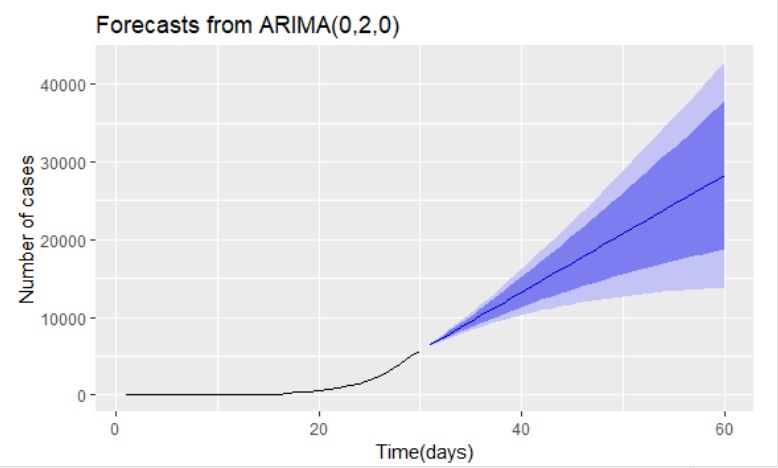
\includegraphics[width=80mm,scale=0.5]{graphs/floridaCases.png}}
            \captionof{figure}{Given the trend in the data, the next 30 days are predicted according to the ARIMA model displaying a largely increasing trend in the number of COVID-19 cases}
        \end{minipage}
        
       
        Figure 2 displays the number of COVID-19 deaths in Florida from March 1st to the 30th of 2020. A 30 day forecast is predicted.
        
        \noindent
        \begin{minipage}{\linewidth}
            \makebox[\linewidth]{
              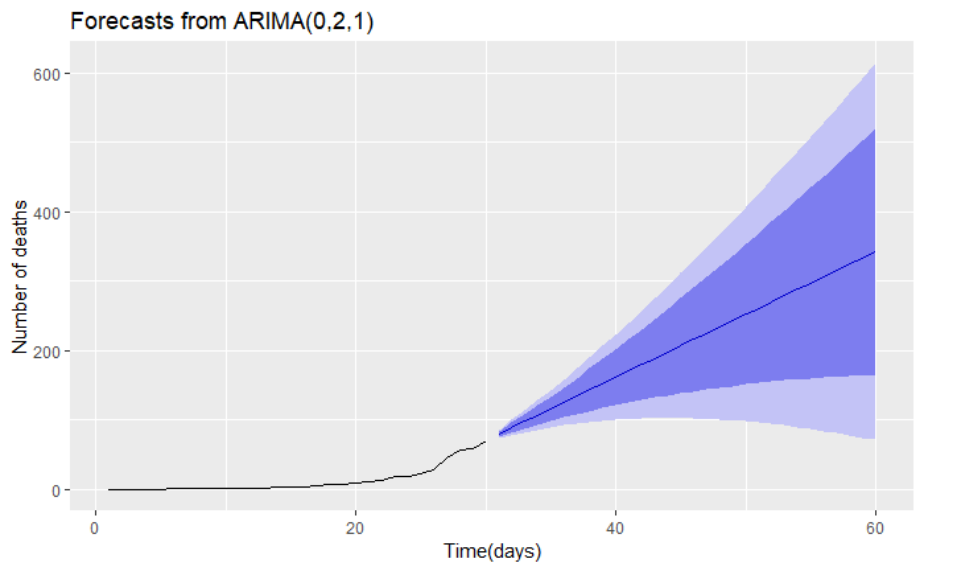
\includegraphics[width=80mm,scale=0.5]{graphs/floridaDeaths.png}}
            \captionof{figure}{Given the trend in the data, the next 30 days are predicted according to the ARIMA model displaying an increasing trend in the number of COVID-19 deaths}
        \end{minipage}
        
        Figure 3 displays the projections for the number of cases in Florida within the next 30 days
        
        \noindent
        \begin{minipage}{\linewidth}
            \makebox[\linewidth]{
              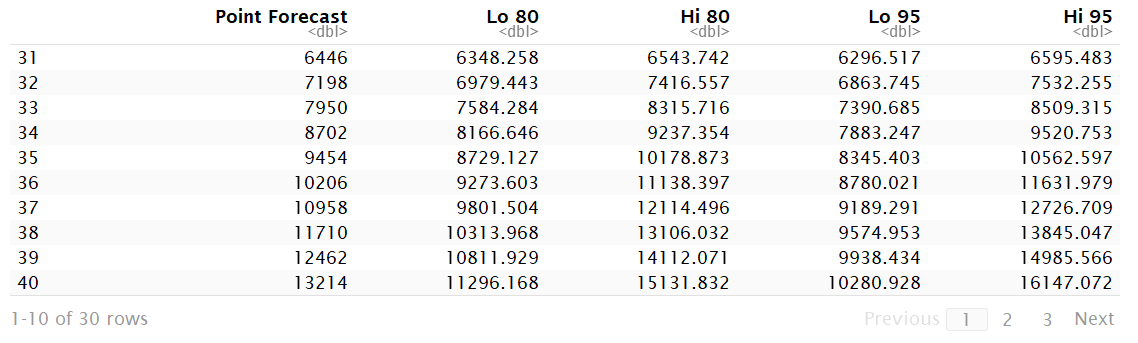
\includegraphics[width=80mm,scale=0.5,height=30mm]{graphs/floridaCases_table.png}}
            \captionof{figure}{Utilizing the ARIMA model, a list of projections for the number of cases in Florida are determined. Lo 80 and Hi 80 refer to the minimum and maximum projections with 80\% confidence respectively. Lo 95 and Hi 95 refer to the minimum and maximum projections with 95\% confidence respectively.}
        \end{minipage}
        
        
        Figure 4 displays the projections for the number of deaths in Florida within the next 30 days
        
        \noindent
        \begin{minipage}{\linewidth}
            \makebox[\linewidth]{
              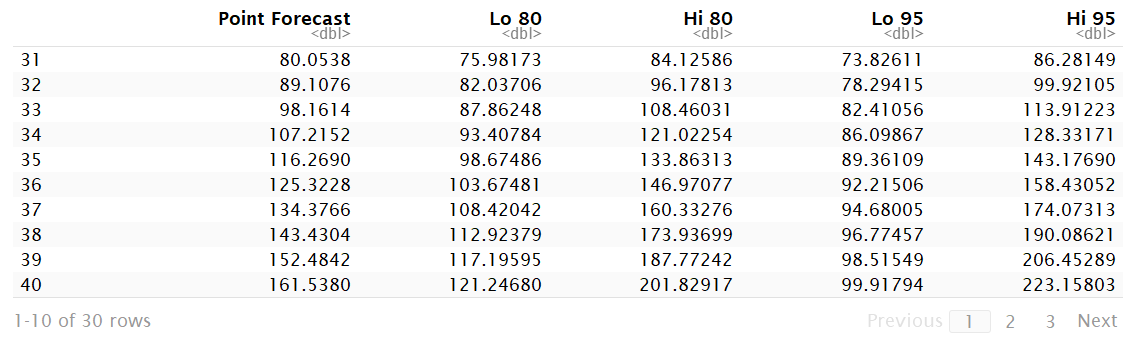
\includegraphics[width=80mm,scale=0.5,height=30mm]{graphs/floridaDeaths_table.png}}
            \captionof{figure}{Likewise, a list of projections for the number of deaths in Florida are determined. Lo 80 and Hi 80 refer to the minimum and maximum projections with 80\% confidence respectively. Lo 95 and Hi 95 refer to the minimum and maximum projections with 95\% confidence respectively.}
        \end{minipage}
    
        Figure 5 displays the number of COVID-19 cases in Florida from March 1st to the 31st of 2020 in a heatmap.
        
        \noindent
        \begin{minipage}{\linewidth}
            \makebox[\linewidth]{
              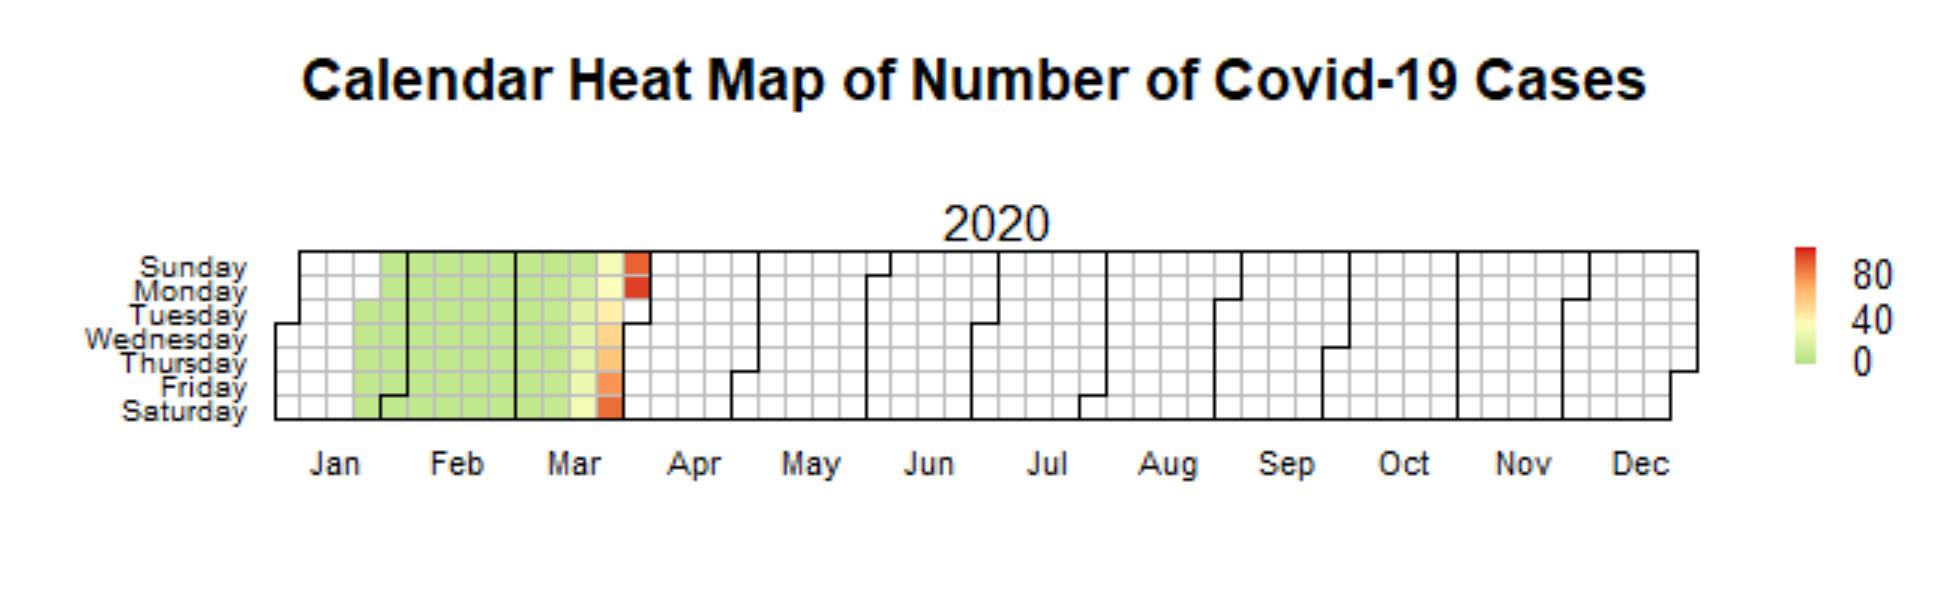
\includegraphics[width=80mm,scale=0.5]{graphs/floridaCasesHeatmap.PNG}}
            \captionof{figure}{The outbreak of covid-19 cases has reach an all time high during the end of March and it doesn't seem to be stopping any time soon.}
        \end{minipage}
    
    \section{Temporal Data Visualization Techniques}
        This section describes some of the more innovative and modern temporal data visualization techniques created in the last few years that have been used to extract patterns and context from time dependent data i.e time series.
        
        \subsection{Popup Plots}
        
            Popup plots employs a 2.5D plot that allow users to
            view different aspects of the data through 3D rotation.
            There are three dimensions to a Popup plot: attributes, landmarks and time. Where time is our independent variable, and the rest are our dependent variables. Attributes concise of measurements such as temperature, volume or any other measurement that changes over time. Landmarks consist of fixed spatial locations. Different points in time are consider as timestamps. Different aspects of the data can be studied by changing the viewing direction which in turn will change the shape of the data\cite{popup-plots}. Here is an illustration of this in action\newline.
        
            \noindent
            \begin{minipage}{\linewidth}
                \makebox[\linewidth]{
                  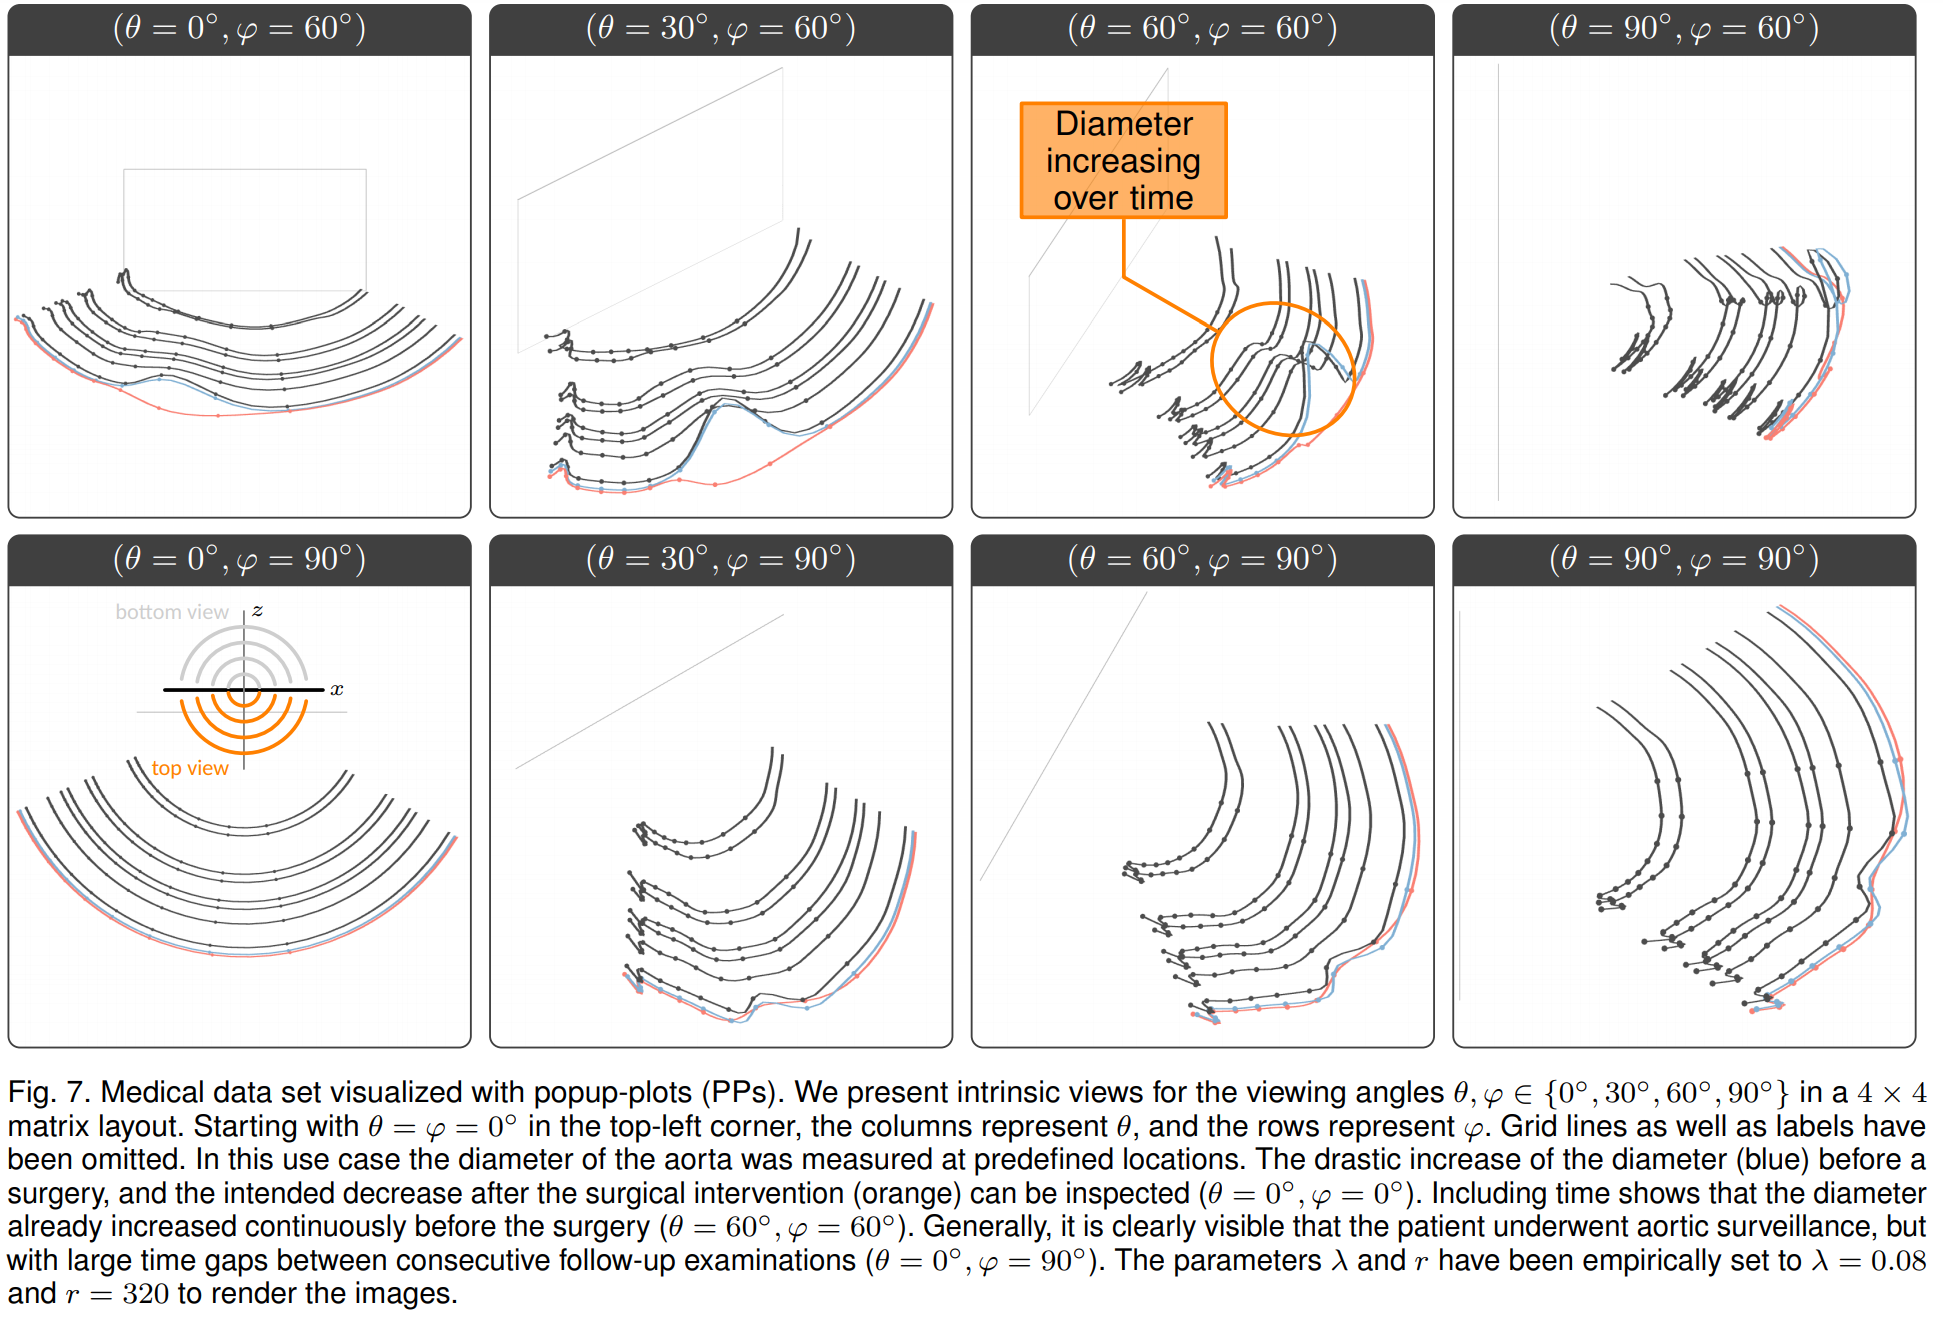
\includegraphics[width=80mm,scale=0.5]{graphs/popup-plot-illustration.PNG}}
                 \captionof{figure}{Shows the lines changing shape and direction as the user rotates plot(2019, p. 9)\newline}
            \end{minipage}
            
            From the bending of the lines, user can deduce which part of data they are looking at and makes it seamless to view the plot from different angles.
            
            \subsection{Space Time Cube}
            
            A space time cube is a visualization technique for visualizing individual movements in space and time. Space time cube comes with a multitude of different operations in order to facilitate information retrieval. Main operations include extracting subparts of the cube, flattening across space and time, transforming the cubes geometry and content etc\cite{space-time-cube}. A full list of all operations is provided in the following illustration. \newline
            
            \noindent
            \begin{minipage}{\linewidth}
                \makebox[\linewidth]{
                  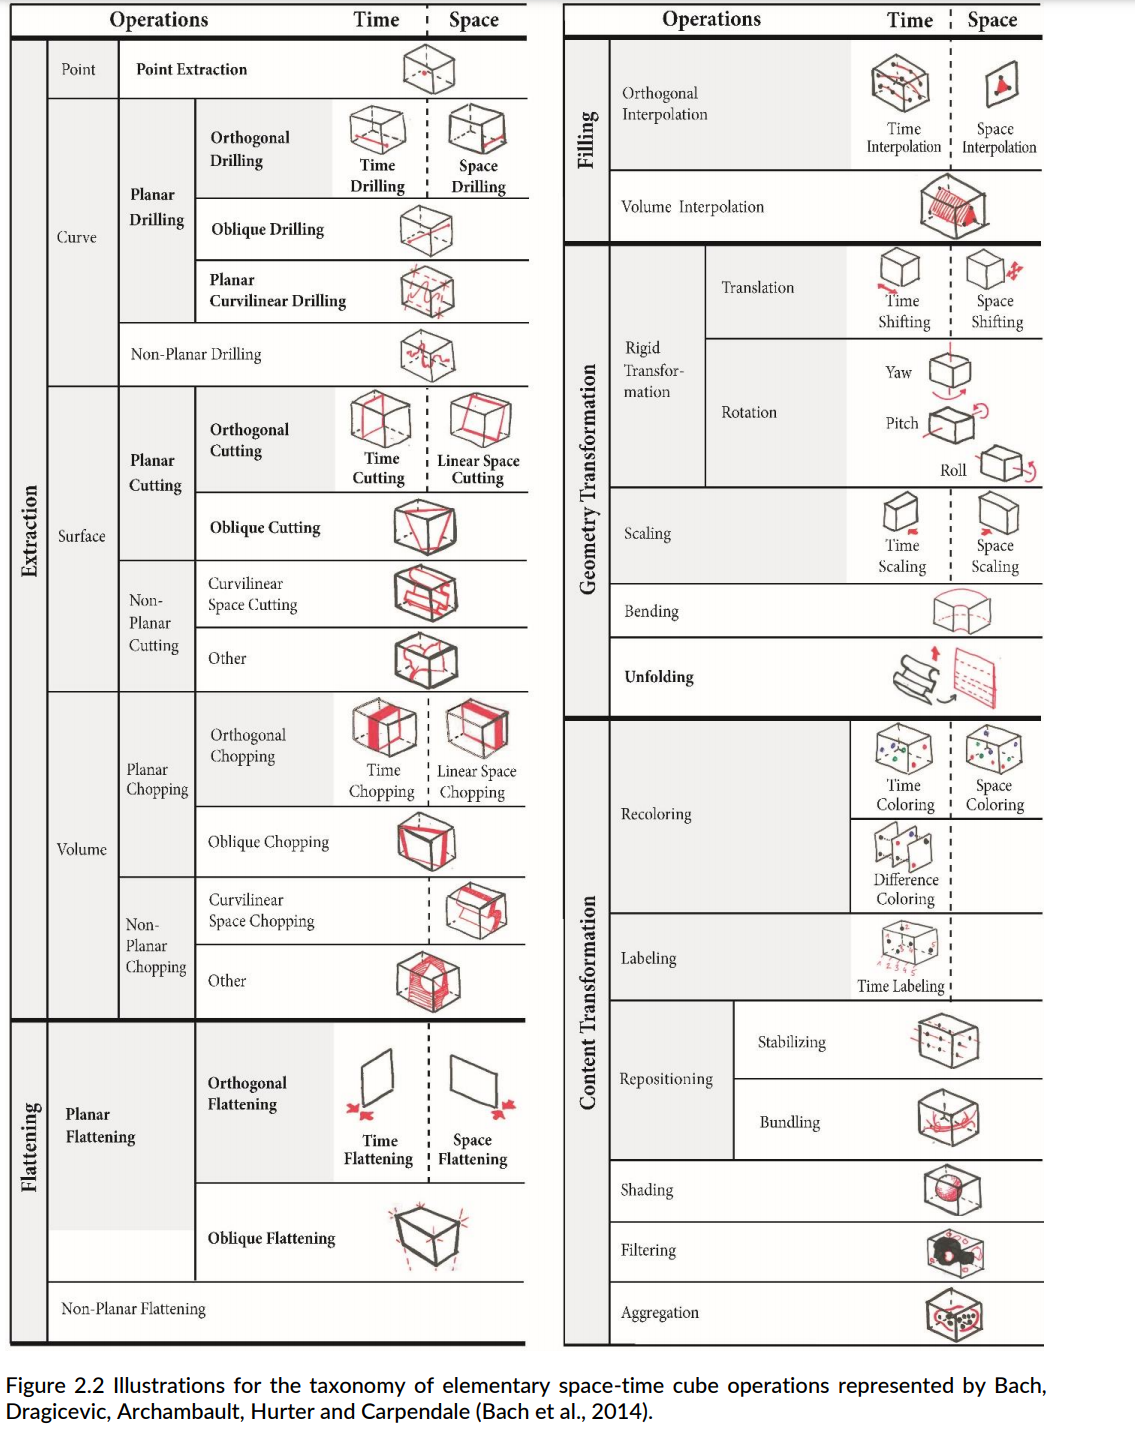
\includegraphics[width=80mm,scale=0.5]{graphs/space-time-cube-operations.PNG}}
                 \captionof{figure}{A full list of all the operations that can be performed on a space time cube(2018, p. 19)\newline}
            \end{minipage}
            
            This representation is very useful and can be used for encoding information such as geolocation, outlining historical landscapes and many more\cite{space-time-cube} for example in a 3D space.
            
    \section{Conclusion}
            
    In summary, temporal data visualization has been an incredibly useful tool for uncovering patterns and trends over time. We explored different techniques used to make the most of temporal data. One of the most useful applications of temporal data visualization is creating prediction models. We explored ARIMA to uncover trends in past data and forecast future values. Our prediction model proved to be quite accurate as the number of cases and deaths followed the numbers reported. Unfortunately, the reports from the government matched with the maximum projection predicted. It seems we are nearing the peak but the number of cases are increasing rapidly. ARIMA was able to help us pinpoint where our data was headed. Although ARIMA is a great tool, machine learning has become a popular and incredibly powerful tool to develop predictions on temporal data. By establishing a neural network, scientists are able to calculate even more accurate predictions.
            
    \clearpage
        
    \begin{thebibliography}{9}
        \bibitem{arima} 
            Prabhakaran, S.(2019). \textit{ARIMA Model - Complete Guide to Time Series Forecasting in Python} Machine Learning Plus. Retrieved from {https://www.machinelearningplus.com/time-series/arima-model-
            time-series-forecasting-python/}
        \bibitem{what-next} 
            Remuzzi, A., \& Remuzzi, G. \textit{COVID-19 and Italy: what next?}. The Lancet: Volume 395, Issue 10231. Retrieved from {https://www.sciencedirect.com/science/article/pii/-
            S0140673620306279}
        \bibitem{popup-plots} 
            Schmidt, J., Fleischmann, D., Preim, B., Brandle, N., \& Mistelbauer, G. (2019). Popup-Plots: Warping Temporal Data Visualization. \textit{IEEE Transactions on Visualization and Computer Graphics, 25} (7), 2443–2457. doi: 10.1109/tvcg.2018.2841385
        \bibitem{nytimes} 
            Smith, M., Yourish, K, \& Allen, J. (2020). \textit{Coronavirus in the U.S.} NY Times. Retrieved from {https://www.nytimes.com/interactive/2020/us/-
            coronavirus-us-cases.html}
        \bibitem{space-time-cube}
            Space-Time Cube Visualization in a Mixed Reality Environment New Approaches to Support Understanding Historical Landscape Changes. (2018). \textit{Technical University of Munich}. Retrieved from {https://www.cartographymaster.eu/wp-content/theses/2018\_TURCHENKO\_Thesis.pdf}
    \end{thebibliography}
\end{document}